\documentclass{article}
\usepackage[utf8]{inputenc}
\usepackage{amsmath}
\usepackage{amsfonts}
\usepackage{amssymb}
\usepackage{graphicx}
\usepackage{geometry}
\usepackage{xcolor}

\newcommand{\inv}{^{-1}}   
\newcommand{\Z}{\mathbb Z}
\newcommand{\R}{\mathbb R}
\newcommand{\Q}{\mathbb Q}
\newcommand{\C}{\mathbb C}
\newcommand{\N}{\mathbb N}

\begin{document}
\pagecolor{black}
\color{white}

\noindent{\bf 1.}

    To make an $8\Omega$, $1W$ resistor, simply connect one pair of $8\Omega$, $\frac14W$ resistors in parallel, then do the same for the other pair, and then connect the two parallel components in series, as shown in the diagram below:

    \begin{center}
    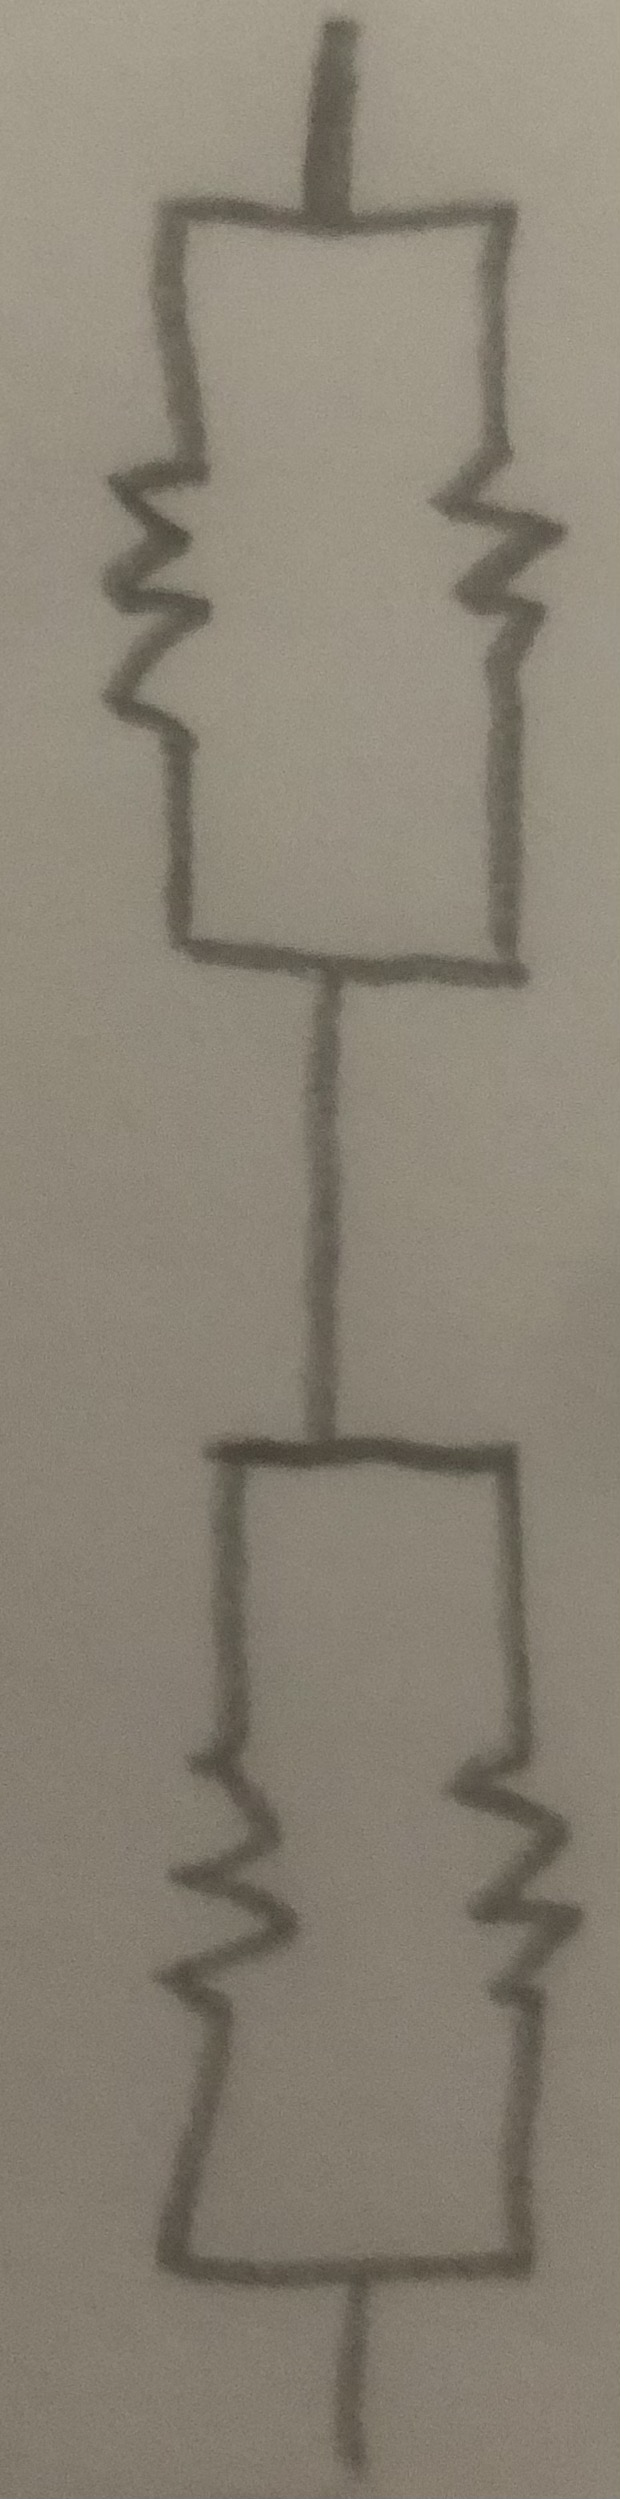
\includegraphics[angle=90,scale=.1]{resistors.jpg}
    \end{center}

\bigskip
\noindent{\bf 2.}

    \begin{center}
    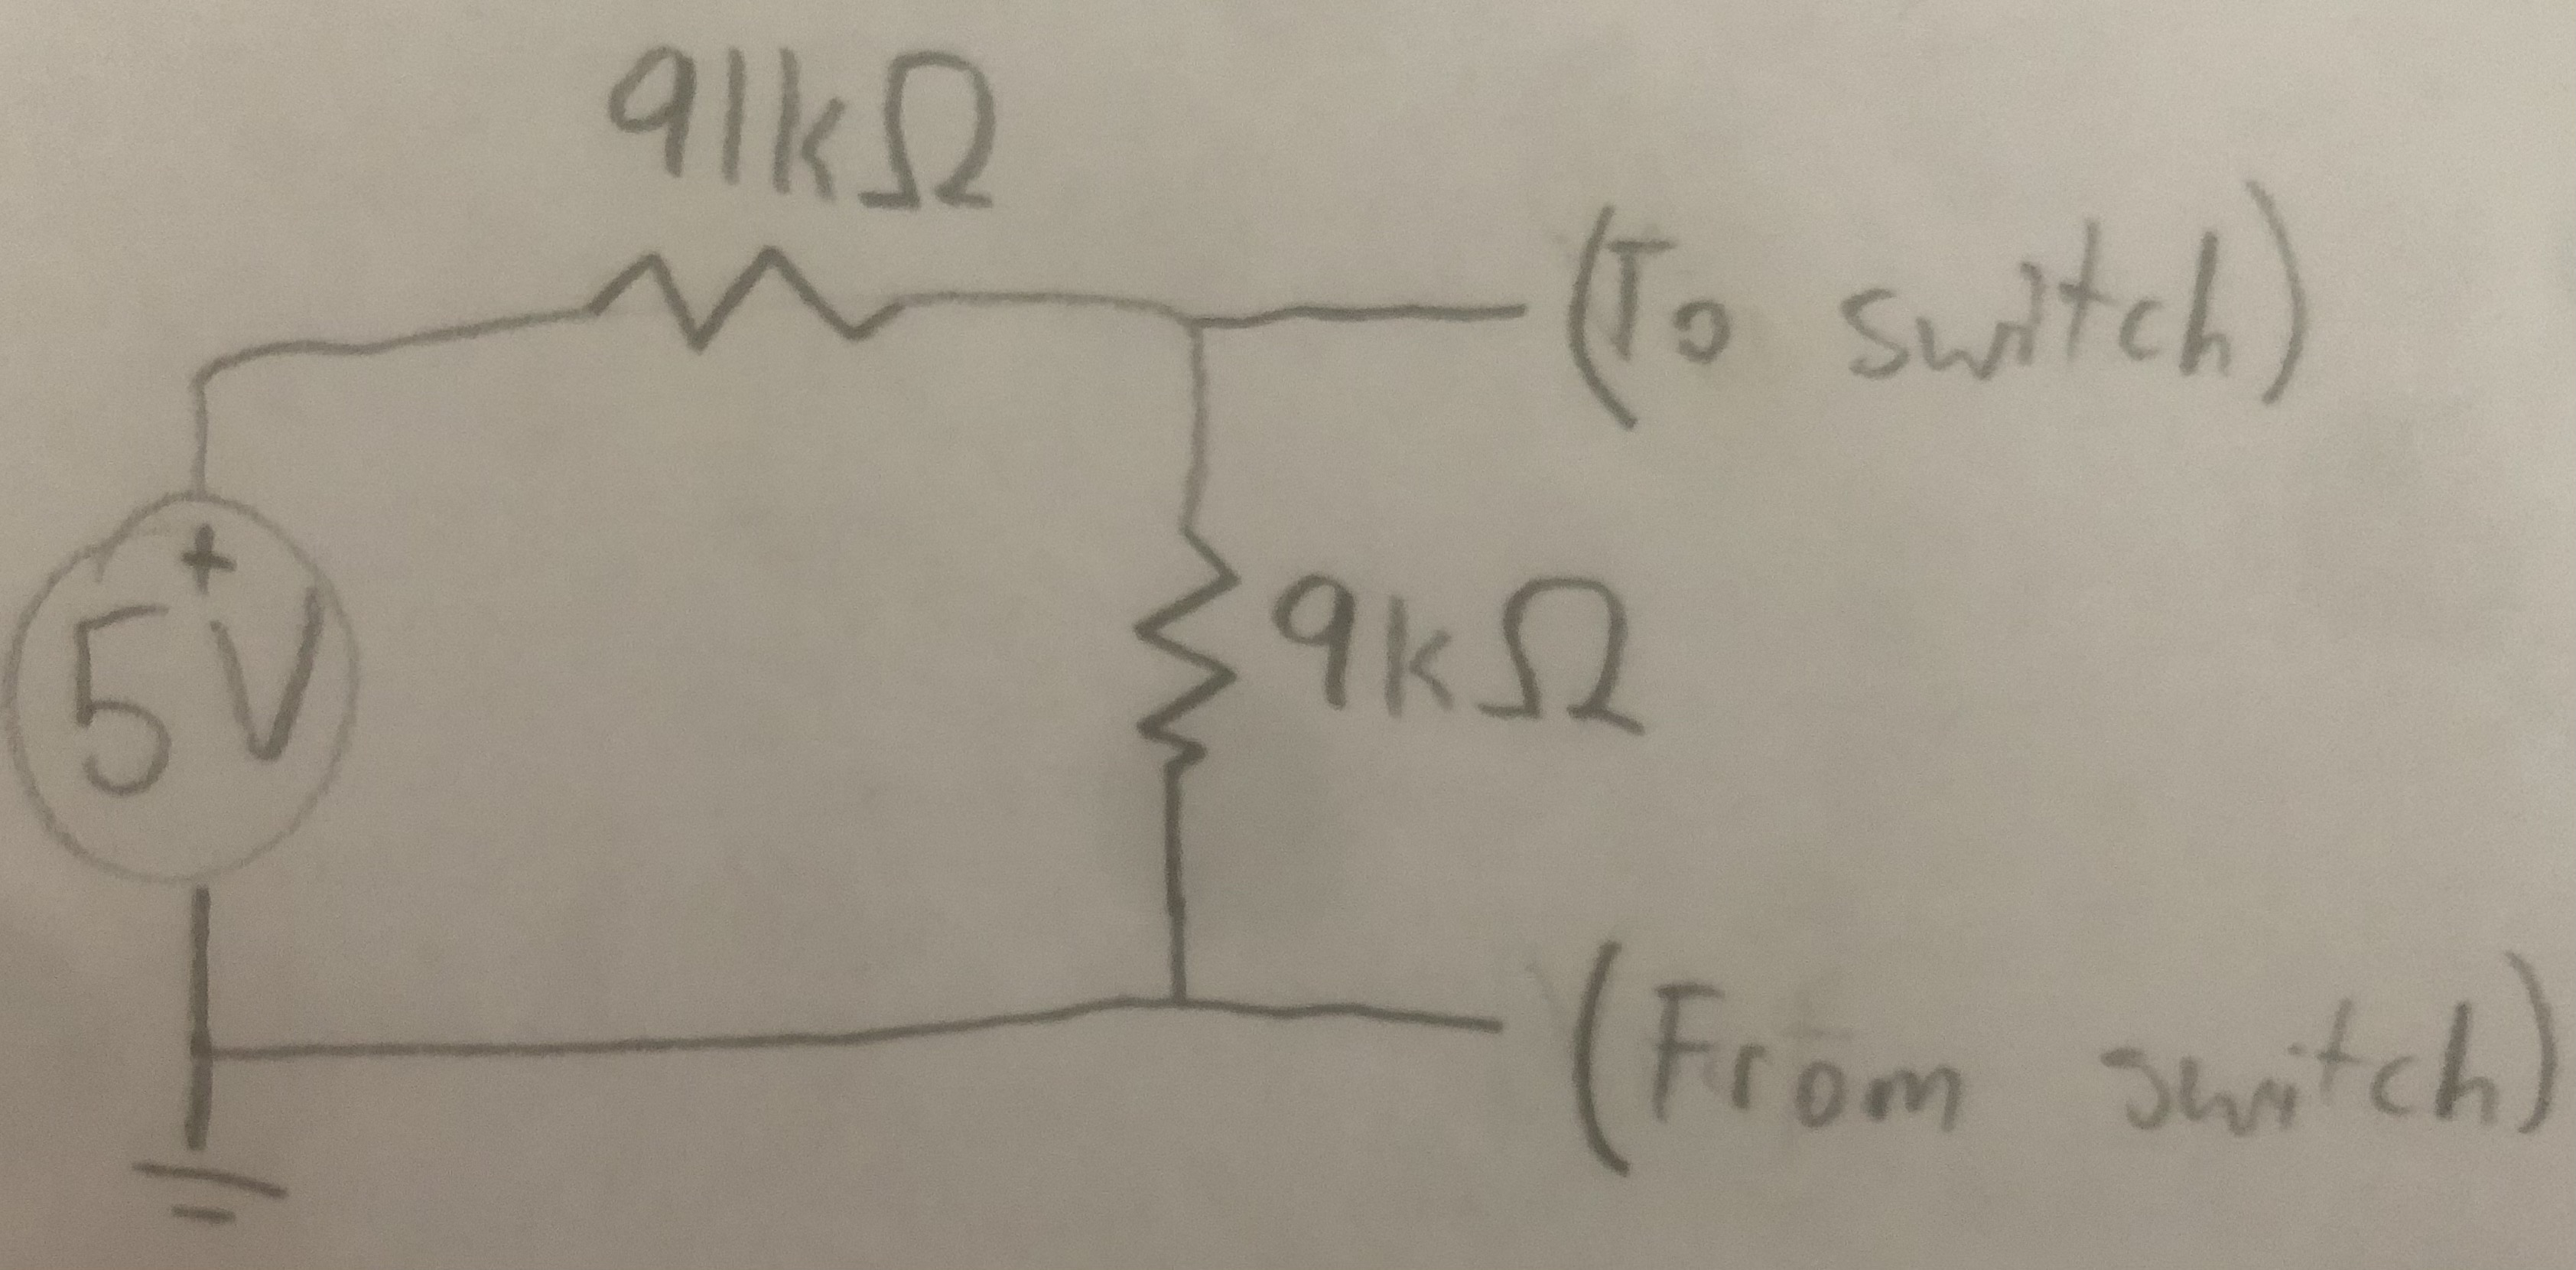
\includegraphics[scale=.1]{switch_circuit.jpg}
    \end{center}

\bigskip
\noindent{\bf 3.}

{\bf (a)} $$2\cdot\frac{1.6}{10}=.32\Omega.$$

\medskip
{\bf (b)}
\begin{align*}
    P &= IV \\
    2000 &= I(115) \\
    \implies I &= \frac{400}{23}\text{A}.
\end{align*}
Thus,
\begin{align*}
    P &= I^2R \\
    2000 &= \left(\frac{400}{23}\right)^2 \cdot R \\
    \implies R &= \frac{529}{80} \\
    &\approx 6.61\Omega.
\end{align*}

\medskip
{\bf (c)} The total resistance of the toaster plus wires is $6.93\Omega$.

\medskip
{\bf (d)}
\begin{align*}
    V &= IR \\
    115 &= I(6.93) \\
    \implies I &\approx 16.59\text{A}.
\end{align*}

\medskip
{\bf (e)}
\begin{align*}
    P_{\text{wires}} &= I^2R \\
                     &= 16.59^2 \cdot .32 \\
                     &\approx 88.07W \\
    P_{\text{toaster}} &= I^2R \\
                       &= 16.59^2 \cdot 6.61 \\
                       &\approx 1819W
\end{align*}

\bigskip
\noindent{\bf 4.}

In the diagram below, let all currents flow to the right through horizontal resistors, and down through vertical resistors.
\begin{center}
    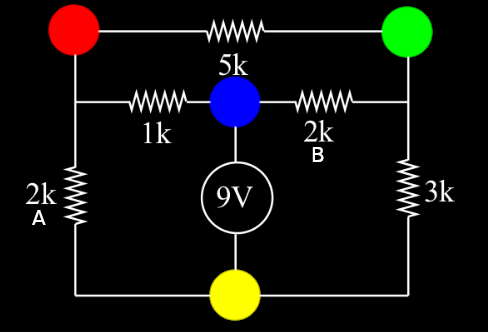
\includegraphics[scale=.65]{circuit.png}
\end{center}




\end{document}
